\section{Multiple Object Tracking}
\label{sec:MultipleObjectTracking}

Our research originally targeted \gls{sot}, especially Siamese trackers. The plan to incorporate multiple objects remained only as a hypothesis to explore later. However, thanks to our comprehensive survey on Siamese tracking~\cite{ondrasovic2021siamese}, we gained enough background knowledge to quickly absorb the newly emerging body of literature on a specific branch of multi-object trackers that exploit Siamese architectures. Our research is focused on Siamese neural networks, whereas the \gls{mot} is dominated by approaches that utilize ``detection \& linking'' while exploiting a wide range of methods, from simple Munkre's algorithm~\cite{munkres1957assignment} through complicated graph formulations~\cite{chen2001motdynamicgraph} to even graph-based convolutional neural networks~\cite{papakis2021gcnnmatch}. Even though there are works that claim the use of Siamese neural networks in \gls{mot}, \egtext{}~\cite{cuan2018deepsiammot}, their utilization serves for the \gls{reid} within the tracking-by-detection philosophy, for which Siamese networks are widely adopted. However, by Siamese tracking, we explicitly mean the type of trackers described in \sectiontext{}~\ref{sec:SingleObjectTracking}. We identified that Siamese-based \gls{mot} is a freshly rising subfield of trackers.

% ##############################################################################
\subsection{Siamese-based Multiple Object Tracking}
\label{ssec:SiameseBasedMultipleObjectTracking}

Shuai~\etal{}~\cite{shuai2020multisiamrcnn} proposed a Siamese-based framework that can simultaneously handle object tracking, detection, and \gls{reid} (\figtext{}~\ref{fig:MultiSiamRCNN}). The unification of all these aspects into a single pipeline is a significant advantage. Fruthermore, the formulation allows the use of any Siamese tracker. Although this tracking system follows an inference pipeline similar to other tracking-by-detection systems, the distinction is that it does so based on features generated by a single network.

% ------------------------------------------------------------------------------
\begin{figure}[!t]
    \centerline{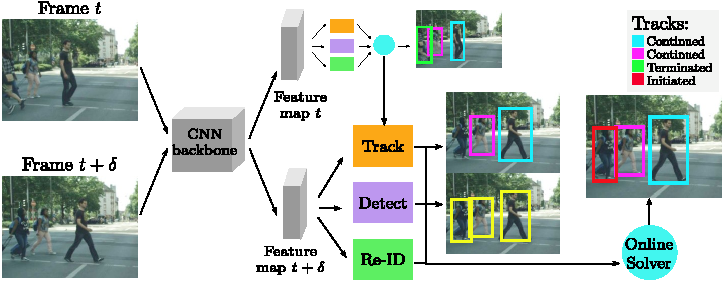
\includegraphics[width=\linewidth]{figures/theoretical_foundations/motsiam_trackrcnn_architecture.pdf}}
    \caption[Siamese \gls{mot} with track R-CNN]{Demonstration of how unification of the detection, tracking and \gls{reid} within a single architecture can be achieved. \externalsrc{\cite{shuai2020multisiamrcnn}}}
    \label{fig:MultiSiamRCNN}
\end{figure}
% ------------------------------------------------------------------------------

A very effective extension aptly dubbed as \gls{siammt} of the often-mentioned came in~\cite{vaquero2021siammt} where the \gls{siamfc} tracker was utilized $n$ exemplars to produce $n$ response maps and, therefore, to perform tracking of $n$ objects simultaneously (\figtext{}~\ref{fig:SiamMTArchitecture}). The incentive to develop this tracker was to address the problem with running a costly detector for every frame to produce detections upon which another performance-demanding linking stage is usually executed. This framework was the first to demonstrate the qualities of a purely deep learning-based, end-to-end tracking pipeline capable of tracking multiple arbitrary objects at once.

% ------------------------------------------------------------------------------
\begin{figure}[!t]
    \centering
    \begin{subfigure}[b]{\textwidth}
        \centering
        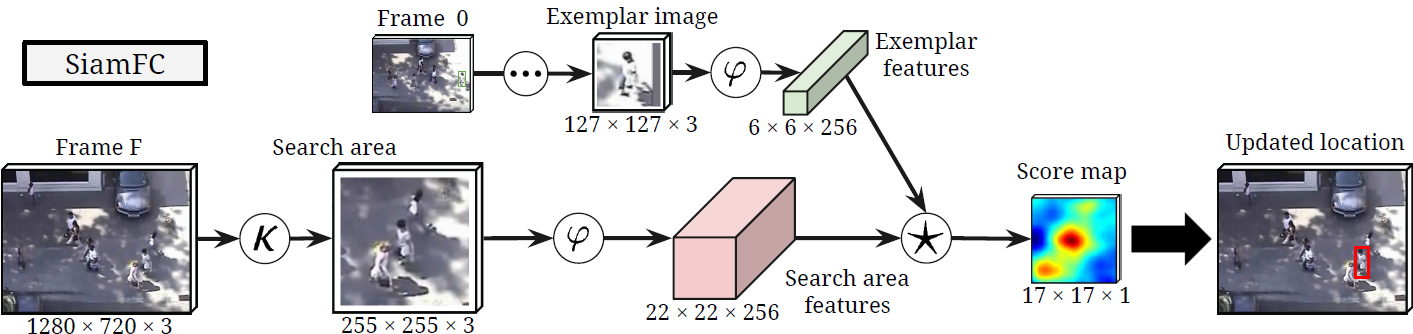
\includegraphics[width=\textwidth]{figures/theoretical_foundations/siammt_orig.png}
        \caption[]{}
    \end{subfigure}
    \begin{subfigure}[b]{\textwidth}
        \centering
        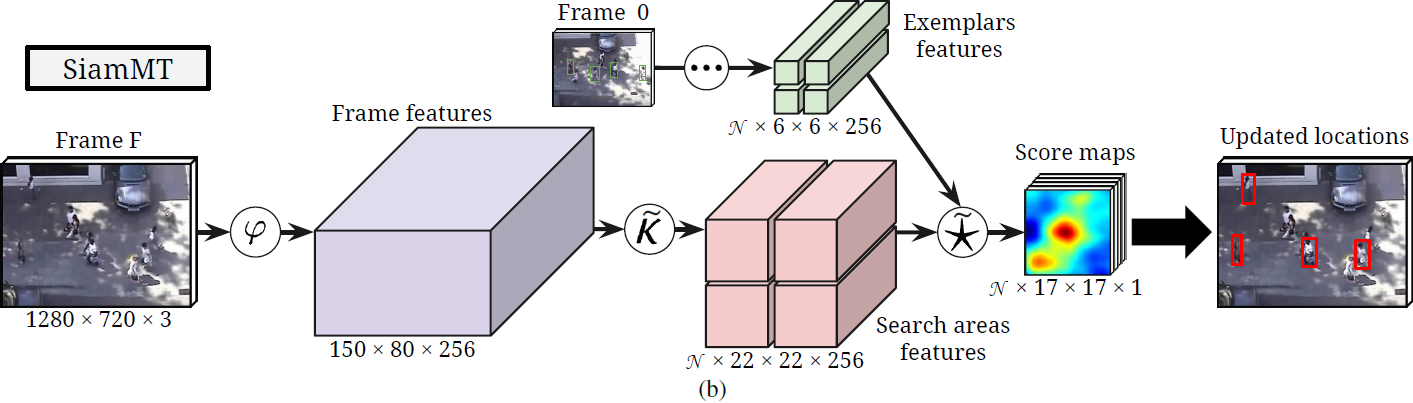
\includegraphics[width=\textwidth]{figures/theoretical_foundations/siammt_new.png}
        \caption[]{}
    \end{subfigure}
    \caption[\gls{siammt} architecture]{The inference phase of the \imgpartdesc{a} \gls{siamfc} to see the difference between the \imgpartdesc{b} \gls{siammt} successor. The \gls{siammt} framework first extracts features of the entire frame via the backbone $\varphi$. The obtained features are cropped and resized using the $\tilde{K}$ operator, utilizing \gls{roi}-align operations. Finally, all these features are combined in the traditional cross-correlation way (slightly adjusted to handle more objects) to produce a multi-object response map. \externalsrc{\cite{vaquero2021siammt}}}
    \label{fig:SiamMTArchitecture}
\end{figure}
% ------------------------------------------------------------------------------

The endeavor to exploit Siamese neural networks to assess the degree of similarity between two objects has spurred a plethora of proposals combining various mechanisms. Lee~\etal{}~\cite{lee2019motfpsn} combined Siamese similarity learning with \glspl{fpn} (\sectiontext{}~\ref{ssec:FeaturePyramidNetworks}). This tracker still follows the path of the tracking-by-detection paradigm, in which the similarity metric between the current detections and existing tracks plays an essential role. In this work, criticism was raised concerning the plain Siamese architectures for not being sufficient for tracking owing to their structural simplicity and lack of motion information. To address the structural simplicity, a \gls{fpsn} was proposed. Then, to overcome the lack of motion information, additional spatiotemporal motion features were added to the \gls{fpsn} module.

As a matter of fact, in our research, we ended up working with \gls{siammot}~\cite{shuai2021siammot} (Section~\ref{sec:SiamMOT}) architecture, which we will introduce in great detail later on. It is a multi-object tracker that encompasses some of the best approaches we have discussed so far into an end-to-end framework, such as Siamese tracker (multi-channel cross-correlation), \gls{rpn} head, \emph{centerness}, feature fusion, and much more.
